\subsection{/home/erik/git/dev/\+Lime\+S\+D\+R-\/\+U\+S\+B\+\_\+\+G\+W/src/txiqmux/compile.tcl File Reference}
\label{txiqmux_2compile_8tcl}\index{/home/erik/git/dev/\+Lime\+S\+D\+R-\/\+U\+S\+B\+\_\+\+G\+W/src/txiqmux/compile.\+tcl@{/home/erik/git/dev/\+Lime\+S\+D\+R-\/\+U\+S\+B\+\_\+\+G\+W/src/txiqmux/compile.\+tcl}}


\subsubsection{Function Documentation}
\index{txiqmux/compile.\+tcl@{txiqmux/compile.\+tcl}!external\+\_\+editor@{external\+\_\+editor}}
\index{external\+\_\+editor@{external\+\_\+editor}!txiqmux/compile.\+tcl@{txiqmux/compile.\+tcl}}
\paragraph[{external\+\_\+editorfilename linenumber }]{\setlength{\rightskip}{0pt plus 5cm}external\+\_\+editor
\begin{DoxyParamCaption}
\item[{}]{filename linenumber }
\end{DoxyParamCaption}
}\label{txiqmux_2compile_8tcl_a44205bac5ddf1d7ed735d8dd5a2ea481}


Definition at line {\bf 15} of file {\bf compile.\+tcl}.

\index{txiqmux/compile.\+tcl@{txiqmux/compile.\+tcl}!q@{q}}
\index{q@{q}!txiqmux/compile.\+tcl@{txiqmux/compile.\+tcl}}
\paragraph[{q}]{\setlength{\rightskip}{0pt plus 5cm}q}\label{txiqmux_2compile_8tcl_a099b3b060154898840f0ebdfb46ec78f}


Definition at line {\bf 52} of file {\bf compile.\+tcl}.

\index{txiqmux/compile.\+tcl@{txiqmux/compile.\+tcl}!r@{r}}
\index{r@{r}!txiqmux/compile.\+tcl@{txiqmux/compile.\+tcl}}
\paragraph[{r}]{\setlength{\rightskip}{0pt plus 5cm}r}\label{txiqmux_2compile_8tcl_a514f1b439f404f86f77090fa9edc96ce}


Definition at line {\bf 48} of file {\bf compile.\+tcl}.



Referenced by {\bf rr()}.



Here is the caller graph for this function\+:\nopagebreak
\begin{figure}[H]
\begin{center}
\leavevmode
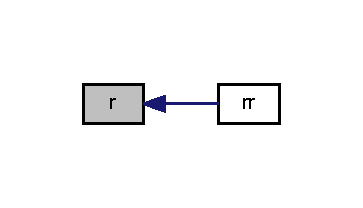
\includegraphics[width=174pt]{d6/d9c/txiqmux_2compile_8tcl_a514f1b439f404f86f77090fa9edc96ce_icgraph}
\end{center}
\end{figure}


\index{txiqmux/compile.\+tcl@{txiqmux/compile.\+tcl}!rr@{rr}}
\index{rr@{rr}!txiqmux/compile.\+tcl@{txiqmux/compile.\+tcl}}
\paragraph[{rr}]{\setlength{\rightskip}{0pt plus 5cm}rr}\label{txiqmux_2compile_8tcl_aeb9279982226a42afdf2860dbdc29b45}


Definition at line {\bf 49} of file {\bf compile.\+tcl}.



References {\bf r()}.



Here is the call graph for this function\+:\nopagebreak
\begin{figure}[H]
\begin{center}
\leavevmode
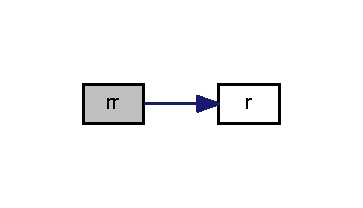
\includegraphics[width=174pt]{d6/d9c/txiqmux_2compile_8tcl_aeb9279982226a42afdf2860dbdc29b45_cgraph}
\end{center}
\end{figure}


